%%%%%%%%%%%%%%%%%%%%%%%%%%%%%%%%%%%%%%%%%%%%%%%%%%%%%%%%%%%%%%%%%%%%%%%%%%%%
% AGUJournalTemplate.tex: this template file is for articles formatted with LaTeX
%
% This file includes commands and instructions
% given in the order necessary to produce a final output that will
% satisfy AGU requirements, including customized APA reference formatting.
%
% You may copy this file and give it your
% article name, and enter your text.
%
%
% Step 1: Set the \documentclass
%
%

%% To submit your paper:
\documentclass[draft]{agujournal2019}
\usepackage{url} %this package should fix any errors with URLs in refs.
\usepackage{lineno}
% \graphicspath{{/Users/jklymak/Dropbox/PW13/satellite/doc/},
%               {/Users/jklymak/Dropbox/PW13/figs/mvp/},
%               {/Users/jklymak/Dropbox/PW13/analysis/mvp/doc/},
%               {/Users/jklymak/Dropbox/PW13/LaPerouse13/doc/},
%               {/Users/jklymak/Dropbox/PW13/auxdata/doc/}}

\graphicspath{{./figs/}}
\DeclareGraphicsExtensions{%
              .pdf,.png}


\usepackage[plain]{fancyref}
% \usepackage[]{hyperref}
%\usepackage[inline]{trackchanges} %for better track changes. finalnew option will compile document with changes incorporated.
\usepackage{soul}
\linenumbers

\draftfalse

\journalname{JGR: Oceans}


\begin{document}

%% ------------------------------------------------------------------------ %%
%  Title
%
% (A title should be specific, informative, and brief. Use
% abbreviations only if they are defined in the abstract. Titles that
% start with general keywords then specific terms are optimized in
% searches)
%
%% ------------------------------------------------------------------------ %%

% Example: \title{This is a test title}

\title{Separation of an upwelling current bounding the Juan de Fuca Eddy}

%% ------------------------------------------------------------------------ %%
%
%  AUTHORS AND AFFILIATIONS
%
%% ------------------------------------------------------------------------ %%

% Authors are individuals who have significantly contributed to the
% research and preparation of the article. Group authors are allowed, if
% each author in the group is separately identified in an appendix.)

% List authors by first name or initial followed by last name and
% separated by commas. Use \affil{} to number affiliations, and
% \thanks{} for author notes.
% Additional author notes should be indicated with \thanks{} (for
% example, for current addresses).

% Example: \authors{A. B. Author\affil{1}\thanks{Current address, Antartica}, B. C. Author\affil{2,3}, and D. E.
% Author\affil{3,4}\thanks{Also funded by Monsanto.}}

\authors{Jody M. Klymak\affil{1,2}, Susan E. Allen\affil{3,4}, Stephanie N. Waterman\affil{3}}


\affiliation{1}{School of Earth and Ocean Sciences, University of Victoria, BC, Canada}
\affiliation{2}{Department of Physcics \& Astronomy, University of Victoria, BC, Canada}
\affiliation{3}{Department of Earth, Ocean and Atmospheric Sciences, University of British Columbia, Vancouver, BC, Canada}
\affiliation{4}{Institute of Applied Mathematics, University of British Columbia, Vancouver, BC, Canada}
%(repeat as many times as is necessary)

%% Corresponding Author:
% Corresponding author mailing address and e-mail address:

\correspondingauthor{J.\ Klymak}{jklymak@uvic.ca}

%% Keypoints, final entry on title page.

%  List up to three key points (at least one is required)
%  Key Points summarize the main points and conclusions of the article
%  Each must be 140 characters or fewer with no special characters or punctuation and must be complete sentences

% Example:
% \begin{keypoints}
% \item	List up to three key points (at least one is required)
% \item	Key Points summarize the main points and conclusions of the article
% \item	Each must be 140 characters or fewer with no special characters or punctuation and must be complete sentences
% \end{keypoints}

\begin{keypoints}
\item The shelf break current along Vancouver Island separates downstream of a submarine bank.
\item Offshore water is drawn onto the shelf and forms a sharp semi-persistent front with the Juan de Fuca Eddy.
\item The Eddy shows evidence of long residence times, and little evidence of deep-water origin.
\end{keypoints}


\begin{abstract}

Comprehensive water column observations of temperature, salinity, and oxygen on the productive southern Vancouver Island shelf offer a unique characterization of processes affecting exchange on the shelf.  A semi-permanent cyclonic recirculation (the Juan de Fuca Eddy) occupies the region in the lee of a bank where the shelf widens abruptly.  The observations indicate that the water in this Eddy is a mixture of offshore water and water from a buoyant coastal current.  The water in the  in the Eddy is well-mixed along a mixing line in $\theta$--$S$ space, though it retains stratification, and is either rapidly mixed (high $\kappa$), or has a long residence time (large $\tau$), such that $(\kappa \tau)^{1/2} \sim 50 -- 100\ \mathrm{m}$.  There is a sharp temperature-salinity front on the offshore side of of this well-mixed water, with the front no more than 1-km wide, and no sign of instabilities. Previous work had hypothesized the role of a spur canyon incising the shelf in feeding water to the Eddy; little evidence of this was found during the observations, however, these were collected during a relaxation and reversal of upwelling winds, which may have slowed the flow of water into the Eddy.  Tidally resolved observations in the spur canyon also show very strong hydraulic flows in the cross-canyon direction accompanied by very high localized mixing rates in 50-m hydraulic jumps possibly exceeding $\kappa \sim 1 \ \mathrm{m^2s^{-1}}$.

Upstream of the Eddy, there is an along-shelf current flowing equatorward with partially mixed water properties compared to the well-mixed water in the Eddy.  The shelf current was observed to separate from the shelf in the lee of a bank, and is replaced by the distinct offshore water mass that forms the offshore front with the Eddy.  The separation event can be seen in sea-surface temperatures in satellite images as tongue of water that is ejected offshore, possibly with the relaxation of upwelling, with the flow heading directly offshore.  The cause of this offshore separation event is not determined, but likely involves instability between the shelfbreak current and the California Undercurrent, and possibly is catalyzed by separation from the abrupt underwater bank at the poleward end of the study region.

\end{abstract}

\section*{Plain Language Summary}

The southern Vancouver Island continental shelf is very productive due to high nutrient input from the Strait of Juan de Fuca and Salish Sea estuarine system, and substantial cross-shelf transport due to the complicated topography.  The estuarine water flows poleward, hugging the coast as the Vancouver Island Coastal Current, and in the summer shelf water flows equatorward.  Trapped between these two currents is the Juan de Fuca eddy, a stagnant region of water that occupies the shelf where it abruptly widens just north of the Strait of Juan de Fuca.

Here we present intensive sampling of the Juan de Fuca eddy region. The observations show the eddy is low in oxygen, and we find has undergone substantial vertical and lateral mixing. This indicates that the waters have a surprisingly long residence time for a coastal feature, and that this region extends the depth of the water column.  In contrast to previous literature we find that the water likely has low oxygen from being used for respiration rather than being pulled from deep in the California Undercurrent.

The sampling also shows a remarkable flow separation of the equatorward shelf current  The current is shown to detach and is pushed offshore. Such events are readily seen in satellite imagery, but the results here indicate that the separation extends the depth of the water column on the shelf, and that this separation may be partially driven by the local bathymetry.  The separation is a very strong cross-shelf exchange event, and likely transports substantial nutrient-rich coastal water offshore to drive productivity in the deeper ocean adjacent to the continental slope.

%% ------------------------------------------------------------------------ %%
%
%  TEXT
%
%% ------------------------------------------------------------------------ %%


%%%%%%%%%%%%%%%%%%%%%%%%%%%%%%%%%%%%%%%%%%%%%%%%%%%%%%%%%%%%%%%%%%%%%
% MAIN BODY OF PAPER
%%%%%%%%%%%%%%%%%%%%%%%%%%%%%%%%%%%%%%%%%%%%%%%%%%%%%%%%%%%%%%%%%%%%%
\section{Introduction}

Cross-shelf exchange is important to the health and productivity of continental shelf regions, where offshore oxygenated water is exchanged with nutrient-rich, but oxygen-depleted nearshore water.  Cross-shelf transport usually requires ageostrophic flow, since geostrophically balanced flow will tend to follow topographic contours, often providing a barrier to lateral exchange \cite{brink16}.  Mechanisms for cross-shelf exchange include internal waves and instabilities in shelf-break fronts.  Most-dramatically, however, topography can drive cross-slope exchanges, often seen most clearly in surface imagery, but occasionally observed \emph{in-situ} \cite{barthetal00}.

Here we present detailed \emph{in-situ} observations from the southern Vancouver Island shelf, collected in summer 2013, and sampled with a rapid profiling vehicle equipped with a CTD and oxygen sensor, supplemented by traditional hydrographic surveys. The shelf has complicated bathymetry \fref{fig:LocMapBoth}, with a somewhat typical shelf poleward of our study site, but then widening in the lee of La Perouse Bank, and then hitting the Juan de Fuca canyon, equatorward.  Water from the strait of Juan de Fuca flows poleward as a buoyant current that hugs the coast \cite{thomsonetal89, hickeyetal91}, while shelf water flows equatorward in the summer under upwelling conditions, both forced by local winds and via tele-connections with the long, homogenous shelves equatorward off Washington and Oregon \cite{hickeyetal91,thomsonkrassovski15,engidaetal16}.  Trapped between these two currents is a region of relatively homogenous water that has been termed the Juan de Fuca Eddy \cite{freelanddenman82,freelandmcintosh89,foremanetal07,macfadyenhickey10}.

A goal of our study was to understand how the Juan de Fuca Eddy persists, and how it exchanges water properties with offshore water.  Low oxygen has previously been found in the Eddy, causing it to be inferred that water in the eddy is upwelled from as deep as 400 m \cite{freelanddenman82,deweycrawford88}.  This inference was based on the oxygen being conservative, and hence having to come from close to the oxygen minimum zone found further offshore \cite{mackasetal87} and lead to hypotheses that perhaps the eddy was fed by waters being drawn up a spur canyon (called the Spur Canyon) via ageostrophic transport from offshore to onshore due to the low pressure in the eddy center \cite{weaverhsieh87}.  Below, we will argue that there is not substantial evidence of such transport, and that oxygen is likely low because of consumption due to respiration.

A second goal was to better understand cross-shore exchange with offshore water.  While the typical schematic of shelf exchange is that there are Ekman layers near the boundaries, there is also evidence of filaments and wholesale separation of shelf currents into the deep ocean, both at this site, and at others.  Such events are important as they tend to transport nutrient rich shelf water out into the open ocean, fueling offshore ecosystems.  Along the Vancouver Island shelf, large filaments or instabilities of the coastal current have been inferred using satellite images \cite{ikedaemery84,thomsongower98}.  Direct observations of such filaments have been made further to the south off Cape Blanco \cite{barthetal00}, and other coasts \cite[e.g.]{relvasbarton05}. Net cross-shore transport of nutrients and chlorophyll have been found in hydrographic surveys off Vancouver Island \cite{mackasyelland99}, and associated with mesoscale features both in geostrophic velocities, and in satellite observations.  The mechanisms driving such separations are poorly understood, but hypotheses include coastal hydraulics \cite{dalebarth01} leading to along-shore trapping of coastal waves,  wind stress curl variations \cite{castelaobarth07}, induced relative vorticity due to stretching of parcels that inertially overshoot their initial isobaths due to a sudden change in downstream bathymetry, and the non-linear breaking of large-scale meanders due to baroclinic instability between the wind-driven current and the California Undercurrent \cite{ikedaetal84, batteen97}.

In this paper we present  observations from 2013 (\fref{sec:Site}), presenting the data in a number of ways to highlight the important processes, with a focus on the offshore side of the eddy region (\fref{sec:Observations}) where we consider the age of the eddy, the steadiness of the front separating the eddy and the offshore water, properties along the spur canyon that was believed to feed the eddy, and finally describe a large offshore tongue of the shelf-break current and its intrusion into the interior.  We discuss the origin of the eddy and the implications of the separating jet (\fref{sec:Summary}).

\section{Site and Methods}
\label{sec:Site}

Observations from three summer cruises in 2013 are discussed here. Two were hydrographic surveys carried out on the \emph{CCGS Tully}, one in June, and the other in late September.  The third was a finescale survey made in the Vancouver Island shelf between 21 and 30 August 2013, aboard the \emph{R/V Falkor}.  The study site was the southern portion of the Vancouver Island Shelf (\fref{fig:LocMapBoth}a), a particularly complicated region due to the bathymetry and varied forcing.

\begin{figure*}[htbp]
  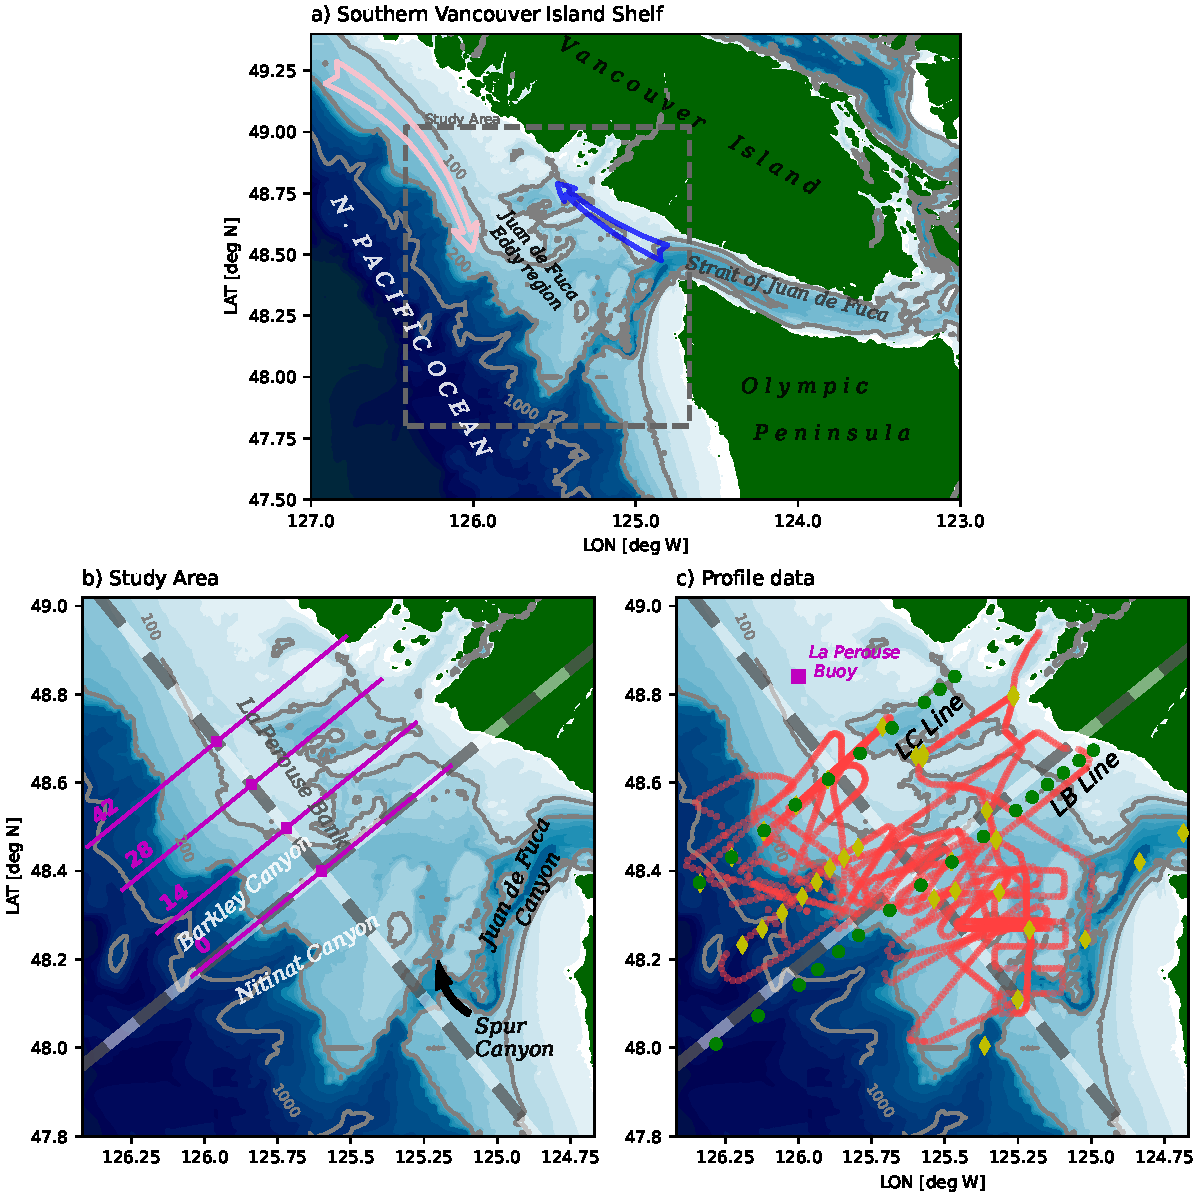
\includegraphics[width=5in]{LocMapBoth.pdf}
  \caption{a) Study site on the Vancouver Island Shelf.  The blue arrow indicates the direction of the Vancouver Island Coastal Current.  The pink arrow indicates southward flow of the coastal upwelling current.  The dashed box indicates the approximate limits of the study area.  b) The study area with hydrographic casts from the La Perouse cruises along the LB and LC Lines are green dots, hydrographic casts during the Falkor cruise indicated in yellow dots, and Moving Vessel Profiler casts as red dots.  The coordinate system used for this paper is shown with alternating grey and white bands at 10-km intervals.}
  \label{fig:LocMapBoth}
\end{figure*}


At the south end of the study site is the Juan de Fuca canyon, which feeds dense water into Juan de Fuca Strait.  This dense water is mixed with fresh water from the Fraser River at the sills and archipelagos further inland, and fluxes out the Strait again, where it turns poleward along Vancouver Island to form the Vancouver Island Coastal Current.  The Juan de Fuca Canyon has a notable spur canyon (Spur Canyon), that incises the shelf towards the north into the study site (\fref{fig:LocMapBoth}b).  The rest of the shelf is punctuated by a series of banks and shallow basins.  Notable is La Perouse bank, running along the shelf from the north, and moving isobaths offshore until it abruptly ends at around 48.5 N. The shelf break is characterized by a series of submarine canyons, in particular Nitnat Canyon and Barkley Canyon.


We consider routine hydrographic surveys along the LB and LC lines, collected aboard the \emph{CCGS Tully} from 2013-05-30 to 2013-05-31  (``June''), and 2013-09-07 to 2013-09-09 (``September'').  These lines span the depths from about 50 m to deep offshore, with casts every 7.5 km across shelf. The data comes from a lowered Seabird 9-11 CTD, with an SBE 43 oxygen sensor.  Oxygen data have been checked against bottle casts, and the CTD corrected for sensor offsets and thermal lags.

We focus on fine-scale surveys carried out from 2013-08-21 to 2013-08-30.  Data were collected from the \emph{R/V Falkor} with an ODIM Brooke-Ocean Moving Vessel Profiler (MVP).  The MVP was equipped with an AML Oceanographic CTD, and a Rinko Oxygen sensor with a 7-s response time foil.  The MVP profiles to depths of 200 m or to within 5 m of the seafloor, whichever is shallower, and drops at a speed of $3\ \mathrm{m\,s^{-1}}$.  Data collection took place while the ship cruised at speeds between 5 and 8 kts, usually at around 6 kts to enable fine horizontal spacing of the casts, with typical spacing less than 800 m.  Data is reported for the downcast, which mostly follows a vertical path.  The rapid speed of the profiling makes the oxygen measurements somewhat coarse, and probably biased due to the phase lag of the sensor, so we treat these largely qualitatively in this paper.

Unfortunately, neither vessel had an operational acoustic Doppler profiler during the cruises with which to make current measurements.

Winds during the cruises were typical for the west coast of Vancouver Island, with upwelling favorable winds during July and early August (\fref{fig:LaPeWind}).  During the finescale cruise, and for the week previous, the winds were intermittently downwelling favorable.  Note that this locale is strongly affected by coastally trapped waves from further south, so doming of near-bottom isopycnals often persists despite local wind forcing \cite{thomsonkrassovski15, engidaetal16}, and takes a finite amount of time to spin down.

\begin{figure*}[htbp]
  \begin{center}
    \includegraphics[width=5.5in]{LaPeWind}
    \caption{
      Wind from the La Perouse buoy \cite{DFOWind2013C46206}.  The vertical direction is along-shelf (chosen as a heading of 315 N), so vectors pointing straight down represent upwelling winds.  .  The wind components has been low-pass filtered to one-day averages.  The timing of the cruises discussed in the paper are shown as colored bands.
      \label{fig:LaPeWind} }
  \end{center}
\end{figure*}


\section{Observations}
\label{sec:Observations}

\subsection{Early and late summer broad-scale surveys}

Hydrographic sections along the LB and LC lines highlight summer conditions on the Southern Vancouver Island Shelf, and indicate some of the features we are focusing on in this paper (\Fref{fig:LaPerouse2013Ctd}).  During both cruises and at both lines there is clear evidence of upwelling, with the $26.4\ \mathrm{kg\,m^{-3}}$ isopycnal reaching from 130 m depth to shallower than 85 m over the shelf.  This dense water tends to be low in oxygen and cool. Further onshore, isopycnals tilt back down, and the water warms, evidence of the Vancouver Island Coastal Current that hugs the coast here.

\begin{figure*}[htbp]
  \begin{center}
     \includegraphics[width=130mm]{LaPerouse2013Ctd}
     \caption{Observations along LC (top three rows) and LB lines (bottom three rows) in Jun (left column) and Sep 2013 (right column).  X is across-shelf distance in the coordinate system shown in \fref{fig:LocMapBoth}. Potential density is contoured every $0.2\ \mathrm{kg\,m^{-3}}$, with the $26.4\ \mathrm{kg\,m^{-3}}$ colored magenta.  Potential temperature, $\theta$, spice anomaly, $\gamma$ and oxygen concentration, $O_2$, are colored for each section.}
     \label{fig:LaPerouse2013Ctd}
  \end{center}
\end{figure*}

The Juan de Fuca Eddy region is along the LB Line (\fref{fig:LaPerouse2013Ctd}, bottom three rows), mostly inshore of 0 km. This water is cooler and lower in oxygen than along the same isopycnal further offshore.  Also note that during the June cruise the water in this region was cooler and more oxygenated than later in the summer during the September cruise.  Near the surface, the isopycnals are domed, but the low-oxygen anomaly extends as high as the thin surface mixed layer.

The water upstream of the Eddy region, along the LC line appears less mixed than the Eddy water.  It does not show as much drawdown of oxygen, and is warmer, at least offshore of La Perouse bank (\fref{fig:LaPerouse2013Ctd}, top three rows).  Water does not appear to make it over La Perouse bank into the basin onshore, or if it does, it does so intermittently.  There appears to be some mixing of the deeper and shallow water near $26.4\ \mathrm{kg\,m^{-3}}$, with the water along this isopycnal becoming cooler and lower in oxygen where it intersects the shelf, consistent with enhanced mixing near the shelf

The $\theta$--$S$ properties show many of the features demonstrated above (\fref{fig:LaPerouse2013TS}a).  Below $26.6\ \mathrm{kg\,m^{-3}}$ or so, the deep water masses are found offshore, and are largely homogenous. Shallower, there are distinct differences between the water found offshore, with it being warmer and saltier than water on the shelf at the same densities. These anomalies are hard to parse directly, so in this paper we use a spice anomaly, relative to a straight line in $\theta$--$S$ space (\fref{fig:LaPerouse2013TS}). This line represents an approximate mixing line for water in the Eddy, and passes the points $7.75\ \mathrm{^oC}$, $30\ \mathrm{psu}$ and $6.6\ \mathrm{^oC}$, $35\ \mathrm{psu}$. Spice anomaly for a given water sample at density $\sigma_{\theta}$ is given by $\gamma = \alpha \left(T - T_0\left(\sigma_{\theta}\right)\right) + \beta \left(S - S_0\left(\sigma_{\theta}\right)\right)$ where $T_0\left(\sigma_{\theta}\right)$, where $S_0\left(\sigma_{\theta}\right)$ are the temperature and salinity along the mixing line at the same density as the water sample, with the sign convention that positive is warmer and saltier than data along the mixing line.

\begin{figure}[htbp]
  \begin{center}
     \includegraphics[width=5in]{LaPerouse2013TS}
     \caption{Potential temperature versus salinity for the La Perouse data shown in \fref{fig:LaPerouse2013Ctd}; potential density is contoured every $0.2\ \mathrm{kg\,m^{-3}}$, with the $26.4\ \mathrm{kg\,m^{-3}}$ colored magenta. A definition of spice anomaly is shown in this plot, and discussed in the text.  The rectangle is the $\theta-S$ range used in \fref{fig:TSdensSpice} below.}
     \label{fig:LaPerouse2013TS}
  \end{center}
\end{figure}

Offshore water tends to be high is absolute spice anomaly (\fref{fig:LaPerouse2013Ctd}, middle rows), with a positive-anomaly layer (red) centered at $26.4\ \mathrm{kg\,m^{-3}}$ sandwiched between negative-anomaly layers above and below.  On the shelf ($-10\, \mathrm{km} < X < 30\, \mathrm{km}$), the distinct $\theta$--$S$ masses are attenuated and much closer to the defined mixing line than the offshore water (closer to white in color).  Hugging the coast ($X > 30\, \mathrm{km}$), is the Vancouver Island Coastal Current, with a negative spice anomaly in June, and a positive anomaly in summer, consistent with seasonal warming.

The June and September cruises are quite similar in water properties, particularly in the offshore waters.  Water has upwelled from deeper depths in September, but has most of the same water mass characteristics as earlier in the year.  The water on the shelf is somewhat warmer than earlier in the year, and by September has started to fall off the mixing line.

In terms of oxygen, both cruises have a similar dichotomy between the onshelf and offshelf water, with water found in the eddy tracking at least $100\ \mathrm{\mu mol\, kg^{-1}}$ lower on the shelf than offshelf (\fref{fig:LaPerouse2013Ctd}, \fref{fig:LaPerouse2013TS}b).  The very deepest water ($S\approx 33.9\ \mathrm{psu}$) on the shelf shows a further $50\ \mathrm{\mu mol\, kg^{-1}}$ drop between June and September along the LB line.

\subsection{Fine-scale surveys}

\subsubsection{Overview}

As shown in \fref{fig:LocMapBoth},  we conducted a large spatial survey of the shelf using the Moving Vessel Profiler, collecting over 2000 CTD casts in a relatively synoptic manner.  This amount of data allows a reasonable census of the water masses that motivated our choice of the mixing line shown in \fref{fig:LaPerouse2013TS}.  Binning in temperature and salinity, we can look at sample frequency of these observations \fref{fig:TSdensSpice}, and we see that there are distinct water masses with few observations between them. Looking along the $26.4\ \mathrm{kg\,m^{-3}}$ isopycnal, we see that there is a large population along the mixing line.  At the opposite extreme, we see that there is a large population with a positive spice anomaly of approximately $0.2\ \mathrm{kg\,m^{-3}}$, representing the offshore water.  Between these two end points there is a third water mass, somewhat indistinct from the offshore water mass, but very distinct from the water mass along the mixing line.  These three water masses exist on deeper and shallower isopycnals as well, but become hard to distinguish from $\theta$--$S$ properties alone as the properties converge near $26.1\,\mathrm{kg\,m^{-3}}$.

% TODO: shallower?

\begin{figure*}[htbp]
  \begin{center}

     \includegraphics[width=3.5in]{TSdensSpice.pdf}
    \caption{Sample density of salinity and potential density data from the cruise, with a logarithmic color scale.  Grey contours are potential density relative to the surface, every $0.1\ \mathrm{kg\,m^{-3}}$, and the magenta contour is the $26.4\ \mathrm{kg\,m^{-3}}$ isopycnal.  Spice anomaly, $\gamma$, is defined as temperature anomaly scaled by the thermal expansion co-efficient, $\alpha$, along isopycnals from the mixing line found in the well-mixed region in the Eddy (white line), in $\mathrm{kg\,m^{-3}}$.
    \label{fig:TSdensSpice}}
  \end{center}
\end{figure*}

In synthetic cross sections of spice anomaly, the Eddy is clearly identifiable as water that is along the straight mixing line, and thus has low-spice anomaly ($\gamma \approx 0\ \mathrm{kg\,m^{-3}}$, \fref{fig:CrossSectionsSpice}c, d).  This signature of well-mixed water extends from the seafloor to approximately 30 m depth, onshore of $x \approx 0\ \mathrm{km}$.  Despite lying along a mixing line, the Eddy water is still stratified.  This well-mixed water contrasts with water directly offshore on the other side of a sharp $\theta-S$ compensated front that is warmer and saltier than the well mixed water ($\gamma > 0.2\ \mathrm{kg\,m^{-3}}$) deeper than $26\,\mathrm{kg\,m^{-3}}$, and colder and fresher shallower.  The thickness of this front is even sharper in individual sections than in these composite sections (see \fref{sec:frontsurvey}).

In contrast, the third population of partially mixed water mass identified in \fref{fig:TSdensSpice} is all found upstream of the Eddy region (\fref{fig:CrossSectionsSpice}a, b) as a weaker spice anomaly ($\gamma \approx 0.1\ \mathrm{kg\,m^{-3}}$, ``pink'' colors).  This water is generally found near the intersection of the upwelling water and La Perouse Bank, and is not as warm as offshore water, indicating some mixing has taken place.  Of note, is that this intermediate water mass appears completely absent in the sections further equatorward (\fref{fig:CrossSectionsSpice}c, d), indicating that it is either mixed away, or that it is advected elsewhere; we argue below that it is advected offshore in a large-scale tongue.

\begin{figure*}[htbp]
  \begin{center}
    \includegraphics[width=6.2in]{CrossSectionsSpice}
    \caption{Synthetic sections of spice anomaly from the MVP data, projected along four lines from poleward (upstream of coastal current) a) to equatorward (downstream); the lines are shown in \fref{fig:LocMapBoth}b).    Isopycnals are contoured every $\sigma_{\theta} = 0.2\,\mathrm{kg\,m^{-3}}$ , with the $\sigma_{\theta} = 26.4\,\mathrm{kg\,m^{-3}}$ isopycnal highlighted in magenta.  Colors are spice anomaly as defined in \fref{fig:TSdensSpice}. "BC" in panel (c) refers to Barkley Canyon.
      \label{fig:CrossSectionsSpice} }
  \end{center}
\end{figure*}

Oxygen section show similar trends, with the low-spice anomaly water having low oxygen saturations, while the strong negative spice anomaly shallower than $\sigma_{\theta} = 26.4\,\mathrm{kg\,m^{-3}}$ has very high oxygen, and the deeper water is also more oxygenated.  Of note is that compared with the coarser sampling along the LC Line (\fref{fig:LaPerouse2013Ctd}), we see that the abrupt transition between offshore and Eddy water is also present in oxygen.

\begin{figure*}[htbp]
  \begin{center}
    \includegraphics[width=6.2in]{CrossSectionsO2}
    \caption{Synthetic sections of Oxygen, approximate percent saturation from the MVP data.
      \label{fig:CrossSectionsO2} }
  \end{center}
\end{figure*}

The spatial patterns are very clear when considering a map-view of properties along the $\sigma_{\theta} = 26.4\,\mathrm{kg\,m^{-3}}$ isopycnal (\fref{fig:SpiceO2264}).  There is a region onshore of the south tip of La Perouse Bank (approximately 44.5 N, 125.75 W), that consists of water that is found along the mixing line (spice anomaly $\gamma \approx 0 \mathrm{kg\,m^{-3}}$) with low oxygen saturations.  Offshore of this region is water that is very warm and salty in comparison ($\gamma > 0.15 \mathrm{kg\,m^{-3}}$), and relatively high in oxygen (saturations of approximately 60\%).  The region between these two water masses is very abrupt, and is concave with respect to the isobaths on the shelf,  stretching from La Perouse Bank to a shallow bank just above the Juan de Fuca canyon (48.3 N and 125.4 W).

Upstream of La Perouse bank and Barkley Canyon, the water along the shelf the weaker spice anomaly of the third water mass ($\gamma \approx 0.1\,\mathrm{kg\,m^{-3}}$, light pink colors).  This water is also somewhat lower in oxygen than water from offshore, though not as depleted as the water in the Eddy.  This water appears to be pushed offshore just upstream of Barkley Canyon, and replaced on the shelf by the warmer offshore water.

\begin{figure*}[htbp]
  \begin{center}
    \includegraphics[width=6.2in]{SpiceO2264}
    \caption{Spatial overview of a) local spice (temperature anomaly on an isopycnal: see text), and b) oxygen saturation on the $\sigma_{\theta} = 26.4\ \mathrm{kg\,m^{-3}}$ isopycnal.  Grey cross-slope lines are cross sections indicated in \fref{fig:CrossSectionsSpice}.  Along-slope grey lines are every 20 km in the cross-slope direction, with $x=0\ \mathrm{km}$ near the 100-m isobath at the north end of the observation area.
   \label{fig:SpiceO2264}
    }
  \end{center}
\end{figure*}

\subsubsection{Frontal survey}
\label{sec:frontsurvey}

A systematic survey through the front between the offshore water and the Eddy water demonstrates the structure of the front (\fref{fig:Frontsurvey}).  The survey started close to shore and passed through the Vancouver Island Coastal Current (along-track 0-10 km).  The coastal current water is buoyant and significantly fresher and cooler than water at the same density near the surface and forms a classic density front with

The front between the offshore water and the ``eddy'' water was passed through 10 times, showing its evolution following the along-shore equatorward flow.  First, as noted in the composite sections, isopycnals slope up from offshore onto the shelf.  This is in agreement with a shelf-break current, though the isopycnals flatten out in the Eddy region.  The front starts out very sharp, (along-track distance $50\ \mathrm{km}$) though two small tendrils can be seen separating from the front on the inshore side.  Similar tendrils are found on the second pass, perhaps a bit more separated from the front ($\approx 80\ \mathrm{km}$), and on the third pass ($\approx 95\ \mathrm{km}$).  Note that these tendrils are made of up partially mixed water.  The subsequent passes have more of this partially mixed water, such that the partially mixed region is up to 5-km wide by the fifth pass ($\approx 150\ \mathrm{km}$).  However, note that the deeper isopycnals retain a sharp front, and indeed the front appears sharp again by the seventh pass at all depths.

There is evidence of some warmer water swirling into Eddy, particularly along isopycnals deeper than $26.4\,\mathrm{kg\,m^{-3}}$.  Regions of warmer (and more oxygenated) water are found in tendrils at these depths (e.g.\ $\approx\,170\ \mathrm{km}$ and $\approx 185\,\mathrm{km}$).

The overall effect is similar to what was seen in the Gulf Stream with similar observations \cite{klymaketal16}; there are two quite distinct water masses, the Eddy water and the offshore water, as seen in the $\theta$--$S$ plot (\fref{fig:Frontsurvey}c). There is only a small population of samples between these two, indicative of substantial isopycnal and vertical mixing, but even these populations are relatively cut off from the main water masses, indicating that they are well-mixed on their own, in short episodic events.

\begin{figure*}[htbp]
  \begin{center}
    \includegraphics[width=6.2in]{Frontsurvey}
    \caption{Data from a survey focusing on the front region (2013-08-28T15:11 to 2013-08-29T09:18) a) spice anomaly along $26.4\,\mathrm{kg\,m^{-3}}$.  Grey-white alternating lines are the coordinate system, with 10-km alternating shades.   b) oxygen saturation; magenta dots correspond to distance along-track. c) density of data points (logscale) in this section of data.  d) cross-section of spice anomaly along track.  Grey isopycnals are contoured every $0.5\,\mathrm{kg\,m^{-3}}$, and the $26.4\,\mathrm{kg\,m^{-3}}$ isopycnal is shown in magenta.  e) cross-section of oxygen saturation.
      \label{fig:Frontsurvey} }
  \end{center}
\end{figure*}

\subsection{Spur Canyon}

The Spur Canyon leading from the Strait of Juan de Fuca has been implicated in allowing dense water to be upwelled into the Eddy.  The seasurface is low in the middle of the Eddy, so water has been hypothesized to move up the Spur Canyon due to ageostrophic motion \cite{weaverhsieh87,freelanddenman82}.  This is difficult to infer from water properties alone.  Three transects up the canyon indicate that deep isopycnals slope up into the canyon (\fref{fig:CanyonPropertiesSpice}, to approximately 30 km).  Across the eddy, isopycnals are largely flat until they intersect the Vancouver Island Coastal Current ($x\approx 80\ \mathrm{km}$).  The deeper isopycnals do not make it into the deeper basin northeast of La Perouse bank ($x\approx 70\ \mathrm{km}$).

\begin{figure*}[htbp]
  \begin{center}
    \includegraphics[width=6.2in]{CanyonPropertiesSpice}
    \caption{Three surveys up the Spur Canyon, where $X$ is along-canyon as defined in the map.  Grey isopycnals are contoured every $0.5\,\mathrm{kg\,m^{-3}}$, and the $26.4\,\mathrm{kg\,m^{-3}}$ isopycnal is shown in magenta.  The seafloor is indicated with the thick black line.
      Map shows the path taken during each survey in chronological order blue, orange, and green.  Magenta line is path taken during a cross-canyon survey (\fref{fig:HydraulicsCanyon}).
      \label{fig:CanyonPropertiesSpice} }
  \end{center}
\end{figure*}

Water properties along the canyon go from offshore water, to Eddy water.  Oxygen behaves in a similar manner, though some of the incoming water has slightly lower oxygen than water inside the eddy (not shown).  Based on these sections, it is difficult to infer water motion up the canyon in particular.

Much of the modified water in the Spur Canyon appears to come from the shelf to the west, but heavily modified by tidal mixing. A repeated tidal survey over the bank on the west side of the canyon shows a strong hydraulic response (\fref{fig:HydraulicsCanyon}) during onshore flow (17:58--21:00).  Dense ocean water passes from the offshore side into the Canyon, and plunges down the side wall before rebounding downstream.  Note that the tide here is largely diurnal, so this onslope flow only occurs once a day.  Given the stratification of $N\approx 6\times10^{-3} \ \mathrm{rad\,s^{-1}}$ and an overturning scale of 50 m, we might expect dissipation rates reaching $\epsilon \sim L^2N^{3} \approx 5\times10^{-4}\ \mathrm{m^2\,s^{-3}}$, which is more than three orders of magnitude higher than dissipation observed west of this location by \citeA{deweycrawford88}.  In terms of a diapycnal diffusivity $\kappa = \gamma \epsilon / N^2 \approx 1\ \mathrm{m^2\,s^{-1}}$, assuming a mixing efficiency of $\gamma=0.2$ The effect on the properties in the canyon is for water to spill over from the offshore front into the canyon during the tide.  This water is rapidly mixed with surrounding water such that its strong offshore spice values are attenuated.

\begin{figure*}[htbp]
  \begin{center}
    \includegraphics[width=4in]{HydraulicsCanyon}
    \caption{Repeated, tide-resolving survey across the Spur Canyon, time is indicated in the upper left of each plot (29 August, 2013).  See magenta line on map \fref{fig:CanyonPropertiesSpice} for location of survey.
      \label{fig:HydraulicsCanyon}
    }
  \end{center}
\end{figure*}

This cross-canyon mixing makes it ambiguous if there is water moving up the canyon or not.  There is indeed a general tendency along the canyon for higher spice water to be found offshore (\fref{fig:CanyonPropertiesSpice}) but it seems likely the source of the higher spice is over the bank rather than water being advected up the canyon.

\subsection{Offshore tongue}

As discussed above, the very sharp T/S front between the well-mixed Eddy water and the offshore water  persists, despite there being considerable partially-mixed water found upstream along the shelf.  The partially-mixed water must go somewhere, and indeed it appears to largely be pushed offshore just upstream of Barkley Canyon (\fref{fig:IsopycnalsDepth}).  There is a tongue of partially mixed ($\gamma$ is pink along $26.4\,\mathrm{kg\,m^{-3}}$) that flows almost due south just west of 126 W. We had trouble crossing the whole tongue with the scale of our surveys, but it is at least 30 km wide. It also appears to end at approximately 48.2 N.  This partially mixed water reaches from relatively shallow isopycnals to at least $26.6\,\mathrm{kg\,m^{-3}}$ (\fref{fig:IsopycnalsDepth}, left panel).  Unfortunately, we cannot track the fate of this water mass because isopycnals tilt down offshore, below the depth limit of the MVP.   The shallower isopycnal appears to have the tongue closer to the shelf than at $26.4\,\mathrm{kg\,m^{-3}}$, indicating strong three-dimensionality to this feature.

This feature is embedded in the larger scale isopycnal tilt caused by the upwelling (\fref{fig:IsopycnalsDepth} right panels), so it is difficult to see dynamically what is driving this offshore push.  One possibility is that it is simple flow separation as the water is not able to make the sharp turn around La Perouse Bank.  Whatever causes it, downstream of the separation, the water is replaced by offshore water with much higher spice values.

\begin{figure*}[htbp]
  \begin{center}
    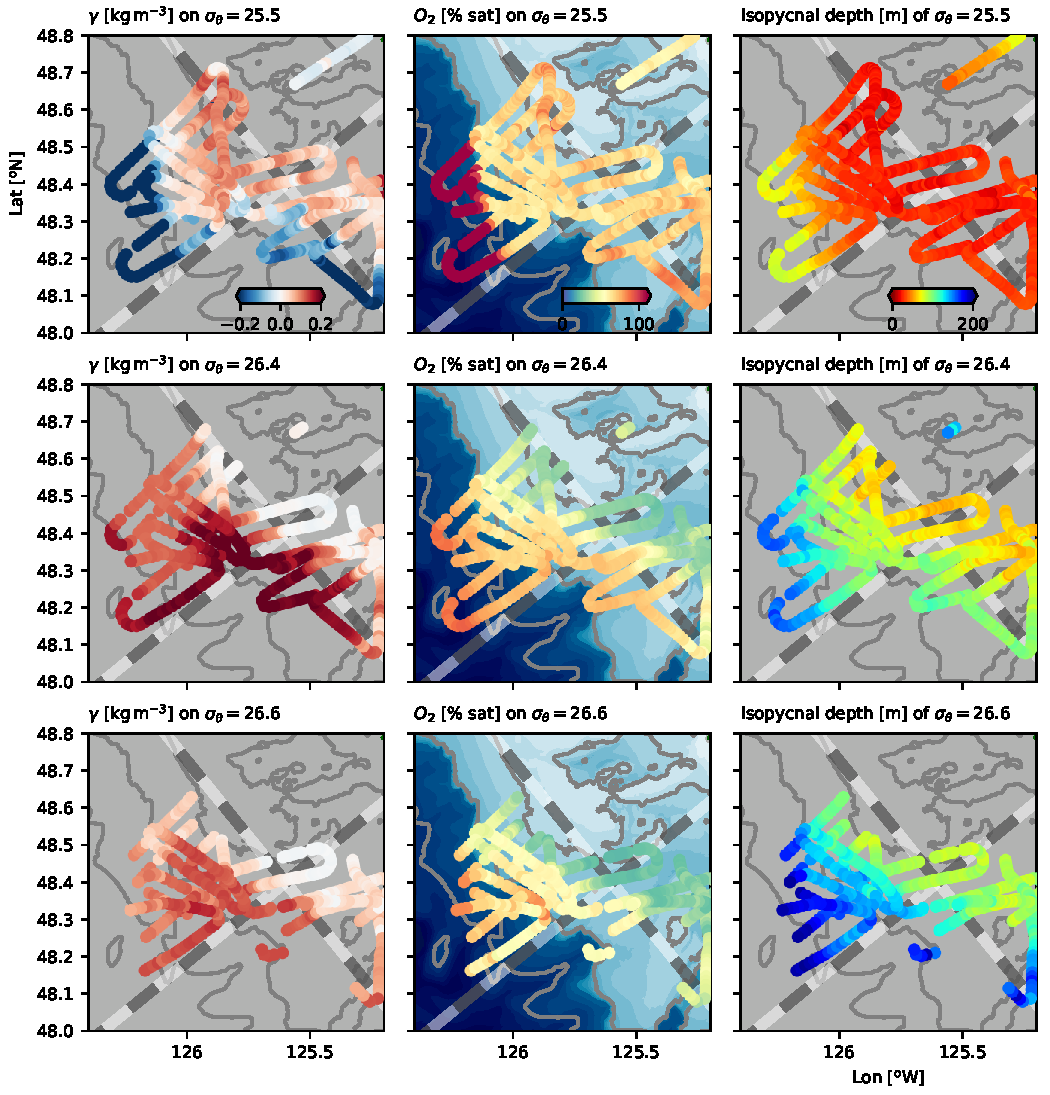
\includegraphics[width=6.2in]{IsopycnalsDepth}
    \caption{Isopycnal slices through showing the vertical structure of the water separating from the shelf, with the first row along $25.5 \,\mathrm{kg\,m^{-3}}$, second along $26.4\,\mathrm{kg\,m^{-3}}$, and the third at $26.6\,\mathrm{kg\,m^{-3}}$.  First column is the spice anomaly, second is oxygen saturation, and the last column is depth of each isopycnal.
      \label{fig:IsopycnalsDepth} }
  \end{center}
\end{figure*}

There is a clear surface expression of the separating tongue in satellite imagery (\fref{fig:SST}).  Water flowing equatorward along the shelf tends to be cooler than offshore water, likely mixing with the colder coming out of the Strait of Juan de Fuca. On Aug 25, there is a cold tongue of water separating from La Perouse bank, crossing isobaths and pointing south at 125.8 W.   There is cooler tendril streaming west at 48 N off the south end of this tongue.  This feature is not as well-developed in the previous image, Aug 21, perhaps indicating that it is an evolving feature.  By 31 Aug, there is no surface expression of the feature, though small tendrils of cooler water can be seen separating from La Perouse Bank.  By Sep-05 the water has significantly warmed, but the offshore anomaly does not appear to have a surface signature.

\begin{figure}
  \begin{center}
    \includegraphics[width=6in]{SSTSnaps}
    \caption{Sea surface temperature snapshots from the observation period.  Grey areas are clouds; dashed gray line is the study area. Depths are contoured in thin gray lines at 200, 150 and 100 m. \cite{L2PMetopA}\label{fig:SST}}
  \end{center}
\end{figure}

Satellite-based surface chlorophyll estimates show the same feature (\fref{fig:ChlA}) demonstrating the advection of high chlorophyll to the west side of the Eddy. It also shows a relatively high-chlorophyll tendril to the west, again exiting the study region at approximately 48 degrees N.  The feature is relatively long-lived, on the order of one month.  Inspection of images before 2013-08-05 were too obscured by clouds, or did not show this feature.  By 2013-09-06, we see the feature fading from the satellite.  However, note that this feature is centered 0.2 degrees of latitude south of tongue that we observe deeper in the water column, again indicating that there is some depth-dependence to the feature.

\begin{figure*}[htbp]
  \begin{center}
    \includegraphics[width=6.2in]{ChlA}
    \caption{Surface chlorophyll density estimated from ocean color \cite{Huetal12,MODISChlL3} over 8-day windows in 4-km bins. Gray regions had too many clouds for acceptable averages.
      \label{fig:ChlA} }
  \end{center}
\end{figure*}


\section{Summary and Discussion}
\label{sec:Summary}

The intensive sampling discussed here has demonstrated a few important features of the South Vancouver Island Shelf.  First, there is a sharp and persistent temperature-salinity compensated front between offshore water, and water that has been termed Eddy water.  This is readily determined in $\theta-S$ space, with the Eddy water lying along a straight mixing line, and the offshore water having a sharp kink centered at $26.4\,\mathrm{kg\,m^{-3}}$.  Second, there was not strong evidence of water moving up the Spur Canyon during our observations, but the Spur Canyon was a site of hydraulic cross-canyon flows in which we infer significant mixing.  Finally, upstream of the Eddy region water in the equatorward shelf current is partially mixed in $\theta-S$ space, and is seen to separate from the shelf at the point of an abrupt bend in an underwater bank.  The water mass crosses isobaths and is ejected into the interior; this can also be observed from satellites.  Thus the water that is offshore of the Eddy appears to have been brought onto the shelf in exchange with this offshore tongue.

\subsection{Age and source of the eddy water}

The source of water and formation of the Juan de Fuca Eddy has received substantial attention, however, the observations of a tight mixing line in $\theta$--$S$ space presented here are a new observation.  The deepest water in the eddy could originate along the $\theta$--$S$ line from approximately 5.5 degrees to 7.5 degrees (\fref{fig:LaPerouse2013TS}a), which in the open ocean spans depths from 420 m to 70 m.  \citeA{mackasetal87} attempted to determine the origin of the water by including oxygen as a third variable to resolve the ambiguous $\theta$--$S$ relation.  However, as \fref{fig:LaPerouse2013TS}b makes clear, oxygen is definitely not a conserved property in the eddy, with concentrations up to $150 \ \mathrm{\mu mol\ kg^{1}}$ lower in the eddy than the water found offshore, and in a way that definitely cannot result from conservative mixing.  As a best guess, if the water in the deepest part of the eddy came from a vertical mixture of the water at $26.5\,\mathrm{kg\,m^{-3}}$ and an equal distance down in density space of $26.7\,\mathrm{kg\,m^{-3}}$, then the deepest water in the eddy would be coming from a depth of 250 m.  This is a typical upwelling depth for coastal flows, and may not require extra input up Spur canyon as posited by \citeA{freelanddenman82}.

We found little evidence of vigorous flow up the Spur Canyon, or if there is, then the mixing in the canyon is quick enough to remove the $\theta$--$S$ signature of offshore water within 20 km of the canyon mouth (\fref{fig:CanyonPropertiesSpice}).  We did find substantial evidence of mixing in the canyon, but the primary route of high-spice water into the canyon appears to be due to tidal flow over the banks on the west side (\fref{fig:HydraulicsCanyon}), rather than evidence of flow up the canyon.  However, it is also of note that upwelling winds had ceased at this point (\fref{fig:LaPeWind}), meaning that the offshore surface pressure gradient may be reduced, leading to reduced ageostrophic upwelling in the canyon.  Whether the cessation of winds would also lead to a reduction of the low sea level height in the center of the eddy is an open question.

There is evidence of aging of the water in the eddy between late spring and late summer (\fref{fig:LaPerouse2013Ctd}), with a reduction of oxygen in the eddy.  If we posited that the reduction was all in the same water, then the oxygen consumption rate over the time between the late-May and early September cruises would be on the order of $0.5\ \mathrm{\mu mol\, kg^{-1} d^{-1}}$.  This seems on the low side of continental upwelling system estimates of apparent oxygen utilization rates, which are between $1$ and $5\  \mathrm{\mu mol\, kg^{-1} d^{-1}}$ \cite{dortchetal94}.   So it seems possible the eddy has enough exchange with the surrounding water for the residence time to be less than the whole time period from late May to September.  Note also that during the June cruise, the water in the Eddy is slightly cooler than the mixing line, and during the September cruise is slightly warmer than the mixing line, so the water in the eddy is evolving seasonally, and probably affected by the water temperature in the Vancouver Island Coastal Current, and the amount of water getting through the front.

The water is  mixed enough in the Eddy that it falls along a mixing line, though it remains vertically stratified. The amount of homogenization is such that either the mixing is very strong, or the water is retained in the eddy for a long time.  The amount of turbulence required to homogenize 100 m of water over 90 days is $\kappa \approx 10^{-3}\ \mathrm{m^2\,s^{-1}}$.  Given that the diffusivity implied in the cross-channel surveys was (very) locally on the order of $\kappa_{\rho} = 10 \ \mathrm{m^2\,s^{-1}}$, this number is not outrageous if we think that such high dissipation is found in $10^{-4}$ of the water column. We can more carefully quantify this by considering a synthetic profile or temperature and salinity based on an offshore profile, extrapolated from the bottom of the 200-m cast to 250 m, assuming that the temperature and salinity at 250 m are $6.2\ \mathrm{[^oC]}$ and $34\ \mathrm{psu}$ respectively (\fref{fig:TSExercise}).  Water at the offshore station was warmer than onshore, so the profile was also linearly interpolated to a surface value of ($12\ \mathrm{^oC}$, $31.6\ \mathrm{psu}$).  The profile was then linearly compressed into a depth range of 150 m representative of the shelf depth in the dense pool, and subjected to mixing with a constant diffusivity of $\kappa = 10^{-3}\ \mathrm{m^2\,s^{-1}}$, with the surface and bottom values pinned under the assumption that the near-bottom source and surface waters are replenished from a large reservoir.  Similar to the naive scaling, the T-S relationship does not approach a straight line until after approximately 60-100 days, or until the mixing affects a vertical length scale of $\lambda = \left(\tau \kappa\right)^{1/2}$ that is greater than $\approx 70\,\mathrm{m}$.

\begin{figure*}[htbp]
  \begin{center}
    \includegraphics[width=4in]{TSExercise}
    \caption{Mixing model assuming constant eddy diffusivity of $\kappa = 10^{-3}\ \mathrm{m^2\,s^{-1}}$ acting on an offshore temperature and salinity profiles compressed from 250 thick to 150 m thick.  Profiles are pinned to the deep value at ($34\ \mathrm{psu}$, $6.2\ \mathrm{^oC}$), and a shallow one at ($31.6\ \mathrm{psu}$, $12\ \mathrm{^oC}$).
      \label{fig:TSExercise} }
  \end{center}
\end{figure*}

The sharpness of the front with the eddy and the offshore water is also intriguing.  It was persistent for the duration of our detailed survey (\fref{fig:SpiceO2264}), and, so far as we can tell with the limited resolution, was present during the La Perouse cruises. There is not any substantial bathymetry blocking the onshore incursion of water at this location, so there must be a dynamic barrier. In contrast, numerical simulations of this region reported by \cite{sahuetal22} using a NEMO 36th-degree regional model  indicate that there is more rapid exchange (order 40 days) between the deep eddy water and the rest of the coastal ocean.  In this model, the region where the eddy resides has velocities equal or greater than other parts of the shelf, and water has an approximate residence time of less than 20 days.  The eddy water in the model does develop a distinct $\theta$--$S$ signature, but not nearly as strong as observed.  It also has a front with the offshore water, but the front is much wider and more gradual than that observed here.

Overall, it would be an improvement to our understanding of the eddy if we could sample the shelf more persistently.  The eddy was already well-formed by the June La Perouse cruise, and seems to evolve slowly during that time.  Capturing its formation, presumably earlier in the spring, and its evolution through the year would be valuable in undertanding retention and exchange on this productive part of the shelf.

\subsection{Offshore exchange of shelf water}

The (apparent) displacement of shelf water from La Perouse Bank is a dramatic departure from geostrophically balanced isobath-following flow..  Eddies have been known to separate from irregular coastal topography, both at the surface \cite{barthetal00}, and deeper in the water column \cite{pellandetal13}.   It has been recognized that instabilities lead to exchange between the open ocean and the shelf at this location \cite{ikedaemery84, ikedaemery84}.   However, observations of the wholesale replacement of shelf water by a new water mass from offshore, is rare. In our situation it is clear that water from as deep as 150 m is separating from the shelf and moving offshore (\fref{fig:SpiceO2264}, \fref{fig:IsopycnalsDepth}).

Satellite imagery makes it clear that there is often an exchange between coastal and deepwater along the Vancouver Island shelf (\fref{fig:SSTLateAug}).  Most years there are three of four large excursions from the shelf into the open ocean, many of them over 100 km long.  This lengthscale is somewhat larger than 60 km inferred for this region by \citeA{ikedaetal84} using a four-layer instability analysis.  It is possible that there is even some spatial locking of these features, with a persistent separation at the north tip of the Island, and a strong tendency for one at 49.5 N.  Our study area also has evidence of a separation in most of the years, with 2011 being the only clear exception. General baroclinic instability of the upwelling front is a possible mechanism to drive offshore exchange \cite<e.g.>{ikedaetal84,durskiallen05}, but this tends to be shallow, with smaller-scale instabilities that will not extend as far into the interior ocean as observed here.  Rather it seems likely that the topographic change engendered by the sudden turn to the east of La Perouse bank catalyses a larger scale instability at this location.  In \citeA{durskiallen05}, when including realistic shelf bathymetry including Heceta Bank, the region around the bank catalyzes intermittent large-scale instabilities similar to the feature here and along the coast \cite{batteen97}.

Large-scale mixing between the shelf and open ocean has been evident since the satellite era.  Here we demonstrate that in this study area the flow is originating on the shelf and separating from the bathymetry and being injected into the interior down to the bottom of the water column.  A  similar observation was made by \citeA{barthetal00} downstream of Cape Blanco, Oregon, where the coastal current was observed to detach from the shelf in the lee of the cape, and flow into the interior.  They hypothesized that as the current moved offshore, it deepened, stretching isopycnals and creating cyclonic relative vorticity that would tend to push the current back onshelf, but then it was caught in the undercurrent and stalled, being pushed offshore. It is also possible that coastally trapped waves in the region experience a hydraulic control, and these meanders are the response \cite{dalebarth01}.

\begin{figure*}[htbp]
  \begin{center}
    \includegraphics[width=6in]{SSTLateAug}
    \caption{
      Available late-August sea-surface temperature from 8-day composites, 2011 to 2021 \cite{MODISSST8d}; missing years had too much cloud cover or no satellite coverage.  \label{fig:SSTLateAug} }
  \end{center}
\end{figure*}

Regardless of the dynamics, the offshore transport is substantial.  If we assume the coastal current is approximately $0.1\ \mathrm{m\,s^{-1}}$ over 100 m in the vertical and 20 km in the horizontal, it represents 0.2 Sv of nutrient- and chlorophyll-rich shelf water transported offshore.  Our observations are a finer detailed representation of the kind of cross-shore transports inferred by \citeA{mackasyelland99} from hydrographic surveys, and definitively show that this water can originate from the shelf from relatively deep depths and be transported offshore.  We do not have velocity measurements for the water that replaces it, but assuming that water also flows along-shelf, there is a large replacement of shelf water with offshore water at this location.  This emphasizes the importance of three dimensional observations and modeling of cross-shelf dynamics when thinking about biological processes on the shelf.

\clearpage
%\section{Here Is Appendix Title}
% will show
% A: Here Is Appendix Title
%
%\appendix
%\section{Here is a sample appendix}

%%%%%%%%%%%%%%%%%%%%%%%%%%%%%%%%%%%%%%%%%%%%%%%%%%%%%%%%%%%%%%%%
%
% Optional Glossary, Notation or Acronym section goes here:
%
%%%%%%%%%%%%%%
% Glossary is only allowed in Reviews of Geophysics
%  \begin{glossary}
%  \term{Term}
%   Term Definition here
%  \term{Term}
%   Term Definition here
%  \term{Term}
%   Term Definition here
%  \end{glossary}

%
%%%%%%%%%%%%%%
% Acronyms
%   \begin{acronyms}
%   \acro{Acronym}
%   Definition here
%   \acro{EMOS}
%   Ensemble model output statistics
%   \acro{ECMWF}
%   Centre for Medium-Range Weather Forecasts
%   \end{acronyms}

%
%%%%%%%%%%%%%%
% Notation
%   \begin{notation}
%   \notation{$a+b$} Notation Definition here
%   \notation{$e=mc^2$}
%   Equation in German-born physicist Albert Einstein's theory of special
%  relativity that showed that the increased relativistic mass ($m$) of a
%  body comes from the energy of motion of the body—that is, its kinetic
%  energy ($E$)—divided by the speed of light squared ($c^2$).
%   \end{notation}




%%%%%%%%%%%%%%%%%%%%%%%%%%%%%%%%%%%%%%%%%%%%%%%%%%%%%%%%%%%%%%%%
%
%  ACKNOWLEDGMENTS
%
% The acknowledgments should list:
%
% 	All funding sources related to this work from all authors
%
% 	Any real or perceived financial conflicts of interests for any
%	author
%
% 	Other affiliations for any author that may be perceived as
% 	having a conflict of interest with respect to the results of this
% 	paper.
%
%   It is also the appropriate place to thank colleagues and other contributors.
%   AGU does not normally allow dedications.

%%%%%%%%%%%%%%%%%%%%%%%%%%%%%%%%%%%%%%%%%%%%%%%

\section*{Open Research}

%Open Research
% AGU requires an Availability Statement for the underlying data needed to understand, evaluate, and build upon the reported research at the time of peer review and publication.

%Additionally, authors should include an Availability Statement for the software that has a significant impact on the research. Details and templates are in the Availability Statement section of the Data & Software for Authors Guidance:
% https://www.agu.org/Publish-with-AGU/Publish/Author-Resources/Data-and-Software-for-Authors#availability

%For physical samples, use the IGSN persistent identifier, see the International Geo Sample Numbers section:
% https://www.agu.org/Publish-with-AGU/Publish/Author-Resources/Data-and-Software-for-Authors#IGSN
%%%%%%%%%%%%%%%%%%%%%%%%%%%%%%%%%%%%%%%%%%%%%%%

\acknowledgments
This section is optional. Include any Acknowledgments here.


%% ------------------------------------------------------------------------ %%
%% References and Citations

%%%%%%%%%%%%%%%%%%%%%%%%%%%%%%%%%%%%%%%%%%%%%%%
%
% \bibliography{<name of your .bib file>} don't specify the file extension
%
% don't specify bibliographystyle

% In the References section, cite the data/software described in the Availability Statement (this includes primary and processed data used for your research). For details on data/software citation as well as examples, see the Data & Software Citation section of the Data & Software for Authors guidance
% https://www.agu.org/Publish-with-AGU/Publish/Author-Resources/Data-and-Software-for-Authors#citation

%%%%%%%%%%%%%%%%%%%%%%%%%%%%%%%%%%%%%%%%%%%%%%%

\bibliography{main}



%Reference citation instructions and examples:
%
% Please use ONLY \cite and \citeA for reference citations.
% \cite for parenthetical references
% ...as shown in recent studies (Simpson et al., 2019)
% \citeA for in-text citations
% ...Simpson et al. (2019) have shown...
%
%
%...as shown by \citeA{jskilby}.
%...as shown by \citeA{lewin76}, \citeA{carson86}, \citeA{bartoldy02}, and \citeA{rinaldi03}.
%...has been shown \cite{jskilbye}.
%...has been shown \cite{lewin76,carson86,bartoldy02,rinaldi03}.
%... \cite <i.e.>[]{lewin76,carson86,bartoldy02,rinaldi03}.
%...has been shown by \cite <e.g.,>[and others]{lewin76}.
%
% apacite uses < > for prenotes and [ ] for postnotes
% DO NOT use other cite commands (e.g., \citet, \citep, \citeyear, \citealp, etc.).
% \nocite is okay to use to add references from your Supporting Information
%



\end{document}



More Information and Advice:

%% ------------------------------------------------------------------------ %%
%
%  SECTION HEADS
%
%% ------------------------------------------------------------------------ %%

% Capitalize the first letter of each word (except for
% prepositions, conjunctions, and articles that are
% three or fewer letters).

% AGU follows standard outline style; therefore, there cannot be a section 1 without
% a section 2, or a section 2.3.1 without a section 2.3.2.
% Please make sure your section numbers are balanced.
% ---------------
% Level 1 head
%
% Use the \section{} command to identify level 1 heads;
% type the appropriate head wording between the curly
% brackets, as shown below.
%
%An example:
%\section{Level 1 Head: Introduction}
%
% ---------------
% Level 2 head
%
% Use the \subsection{} command to identify level 2 heads.
%An example:
%\subsection{Level 2 Head}
%
% ---------------
% Level 3 head
%
% Use the \subsubsection{} command to identify level 3 heads
%An example:
%\subsubsection{Level 3 Head}
%
%---------------
% Level 4 head
%
% Use the \subsubsubsection{} command to identify level 3 heads
% An example:
%\subsubsubsection{Level 4 Head} An example.
%
%% ------------------------------------------------------------------------ %%
%
%  IN-TEXT LISTS
%
%% ------------------------------------------------------------------------ %%
%
% Do not use bulleted lists; enumerated lists are okay.
% \begin{enumerate}
% \item
% \item
% \item
% \end{enumerate}
%
%% ------------------------------------------------------------------------ %%
%
%  EQUATIONS
%
%% ------------------------------------------------------------------------ %%

% Single-line equations are centered.
% Equation arrays will appear left-aligned.

Math coded inside display math mode \[ ...\]
 will not be numbered, e.g.,:
 \[ x^2=y^2 + z^2\]

 Math coded inside \begin{equation} and \end{equation} will
 be automatically numbered, e.g.,:
 \begin{equation}
 x^2=y^2 + z^2
 \end{equation}


% To create multiline equations, use the
% \begin{eqnarray} and \end{eqnarray} environment
% as demonstrated below.
\begin{eqnarray}
  x_{1} & = & (x - x_{0}) \cos \Theta \nonumber \\
        && + (y - y_{0}) \sin \Theta  \nonumber \\
  y_{1} & = & -(x - x_{0}) \sin \Theta \nonumber \\
        && + (y - y_{0}) \cos \Theta.
\end{eqnarray}

%If you don't want an equation number, use the star form:
%\begin{eqnarray*}...\end{eqnarray*}

% Break each line at a sign of operation
% (+, -, etc.) if possible, with the sign of operation
% on the new line.

% Indent second and subsequent lines to align with
% the first character following the equal sign on the
% first line.

% Use an \hspace{} command to insert horizontal space
% into your equation if necessary. Place an appropriate
% unit of measure between the curly braces, e.g.
% \hspace{1in}; you may have to experiment to achieve
% the correct amount of space.


%% ------------------------------------------------------------------------ %%
%
%  EQUATION NUMBERING: COUNTER
%
%% ------------------------------------------------------------------------ %%

% You may change equation numbering by resetting
% the equation counter or by explicitly numbering
% an equation.

% To explicitly number an equation, type \eqnum{}
% (with the desired number between the brackets)
% after the \begin{equation} or \begin{eqnarray}
% command.  The \eqnum{} command will affect only
% the equation it appears with; LaTeX will number
% any equations appearing later in the manuscript
% according to the equation counter.
%

% If you have a multiline equation that needs only
% one equation number, use a \nonumber command in
% front of the double backslashes (\\) as shown in
% the multiline equation above.

% If you are using line numbers, remember to surround
% equations with \begin{linenomath*}...\end{linenomath*}

%  To add line numbers to lines in equations:
%  \begin{linenomath*}
%  \begin{equation}
%  \end{equation}
%  \end{linenomath*}



